\documentclass[11pt]{article}
\usepackage{amsmath, amssymb, amsthm}
\usepackage{geometry}
\usepackage{hyperref}
\usepackage{booktabs}
\usepackage{enumitem}
\usepackage[dvipsnames]{xcolor}
\usepackage{tcolorbox}
\usepackage{listings}

\geometry{margin=1.05in}
\hypersetup{colorlinks=true, linkcolor=blue!60!black, urlcolor=blue!60!black}

\newcommand{\eps}{\varepsilon}
\newcommand{\code}[1]{\texttt{#1}}
\newcommand{\R}{\mathbb{R}}
\newcommand{\dv}{\nabla\cdot}
\newcommand{\Nc}{\mathcal{N}}
\newcommand{\Kc}{\mathcal{K}}
\newcommand{\hphi}{\hat\varphi}
\setlist[itemize]{leftmargin=1.4em, itemsep=2pt}
\setlist[enumerate]{leftmargin=1.8em, itemsep=3pt}

\lstset{basicstyle=\ttfamily\small, columns=fullflexible, keepspaces=true,
        frame=single, framerule=0.3pt, rulecolor=\color{gray!60}, xleftmargin=4pt,
        breaklines=true, language=Python, showstringspaces=false}

\newcounter{ex}
\newenvironment{ex}[1]{\refstepcounter{ex}\par\medskip\noindent\textbf{Exercise \theex}\ \ \textit{#1}\par\nopagebreak\smallskip}{\par\medskip}
\newtcolorbox{codebox}[1]{colback=green!4!white, colframe=green!40!black, title=Code check: \code{#1}, fonttitle=\bfseries\small, boxrule=0.5pt, arc=1pt, left=4pt, right=4pt, top=3pt, bottom=3pt}
\newtcolorbox{goal}{colback=orange!6!white, colframe=orange!70!black, boxrule=0.5pt, arc=1pt, left=4pt, right=4pt, top=3pt, bottom=3pt}

\title{Worksheet: the Gushchin construction\\ for the grid solver}
\author{Companion to \code{python/shared/mixture\_sb.py}, \code{paper\_route\_sb.py}\\
and \code{docs/sb\_primer.tex}, Sections 9--10}
\date{24 October 2026}

\begin{document}
\maketitle

\begin{goal}
\textbf{Goal for today.} Be able to (i) state in one sentence why a constructed pair has a
known Schr\"odinger bridge, (ii) derive every formula in the two reference classes by
hand, (iii) audit each line of the code against your derivation, and (iv) run the 2D split
example and the ring example through the GPU solver and know what error to expect.
Parts A--E are pen, paper and plain numpy (no JAX, runs on the Mac). Part F is the GPU plan.
Answers are in Appendix~\ref{sec:answers}; try each exercise before looking.
\end{goal}

\section*{Conventions}
Solver PDE: $\partial_t\rho+\dv m=\eps\Delta\rho$, $m=\rho v$, on $[0,1]^d$ with no-flux
walls, $t\in[0,1]$. Reference SDE $dX=\sqrt{2\eps}\,dW$, so the heat kernel over time $t$
is $\Nc(\cdot;\,x,\,2\eps t\,I)$. We write $\sigma^2:=2\eps$. The paper's regularization
$\epsilon_{\rm p}$ equals $\sigma^2=2\eps$: \emph{their} $\eps$ is twice \emph{ours}. The
code writes \code{2*eps} wherever $\sigma^2$ appears. Primer section numbers refer to
\code{sb\_primer.pdf}.

\section*{Part A. The one fact everything rests on}

\begin{ex}{The Gibbs form (primer Prop.\ 5.4 and Prop.\ 9.1, paper Thm.\ 3.2).}
Write down the plan
\[
  \pi(x,y)=\hphi(x)\,\Kc_\sigma(x,y)\,\varphi(y),\qquad
  \Kc_\sigma(x,y)=\Nc(y;x,\sigma^2I),
\]
for two positive functions $\hphi,\varphi$ with $\iint\pi=1$. Compute its two marginals in
terms of $\hphi$, $\varphi$ and the heat flow, and name the two functions
\[
  \varphi_0(x):=\int\Kc_\sigma(x,y)\varphi(y)\,dy,\qquad \hphi_1(y):=\int\hphi(x)\Kc_\sigma(x,y)\,dx .
\]
State in one sentence why $\pi$ is the entropic-optimal plan between its own marginals.
(Hint: the optimal plan is characterized by having the form ``function of $x$ times kernel
times function of $y$''; nothing else is needed.)
\end{ex}

\begin{ex}{From the static plan to the bridge.}
Define the backward and forward heat flows of the two factors,
\[
  \varphi_t:=\Kc_{\sigma\sqrt{1-t}}*\varphi \ \ (\partial_t\varphi_t=-\eps\Delta\varphi_t,\ \varphi_1=\varphi),\qquad
  \hphi_t:=\Kc_{\sigma\sqrt{t}}*\hphi \ \ (\partial_t\hphi_t=+\eps\Delta\hphi_t,\ \hphi_0=\hphi),
\]
and set $\rho_t:=\varphi_t\hphi_t$, $v:=\sigma^2\nabla\log\varphi_t=2\eps\nabla\varphi_t/\varphi_t$.
Show by direct differentiation that
\[
  \partial_t\rho_t+\dv(\rho_t v)=\eps\Delta\rho_t .
\]
This is the computation that ties the construction to \emph{our} PDE; do it fully.
(Expand $\Delta(\varphi\hphi)=\hphi\Delta\varphi+2\nabla\varphi\!\cdot\!\nabla\hphi+\varphi\Delta\hphi$
and $\dv(\rho v)=2\eps\,\dv(\hphi\nabla\varphi)$.)
Then check $\rho_0=\hphi\varphi_0$ and $\rho_1=\varphi\hphi_1$ match Exercise~1.
\end{ex}

\begin{ex}{Which object is which.}
Fill in the table from memory, then check against the primer's symbol table (Sec.\ 11).
\begin{center}\small
\begin{tabular}{@{}lll@{}}
\toprule
object & paper's name/symbol & code \\
\midrule
$\varphi$ (the $y$-side factor) & $\exp(f^*/\epsilon_{\rm p})$, LSE potential, eq.\ (15) & \code{phi(1.0, .)}, args \code{(w, b, Q)}\\
$\varphi_0$ & \rule{2.2cm}{0.3pt} & \rule{2.2cm}{0.3pt}\\
$\hphi$ & \rule{2.2cm}{0.3pt} & \rule{2.2cm}{0.3pt}\\
$\pi^*(y|x)$ & \rule{2.2cm}{0.3pt} & \rule{2.2cm}{0.3pt}\\
$v=\sigma^2\nabla\log\varphi_t$ & \rule{2.2cm}{0.3pt} & \rule{2.2cm}{0.3pt}\\
\bottomrule
\end{tabular}
\end{center}
\end{ex}

\section*{Part B. The two Gaussian identities}

Everything explicit below comes from two facts about $\Nc(z;\mu,\Sigma)$.

\begin{ex}{Convolution rule.}
Show $\Nc(\cdot;\mu,\Sigma)*\Nc(\cdot;0,\tau^2I)=\Nc(\cdot;\mu,\Sigma+\tau^2I)$ (sum of
independent Gaussians). Conclude: the heat flow with generator $\eps\Delta$ over a time
$s$ adds $2\eps s\,I$ to every covariance. Which sign of $s$ goes with $\varphi_t$ and
which with $\hphi_t$? Write both $\varphi_t$ and $\hphi_t$ for mixtures
$\varphi=\sum_nw_n\Nc(\cdot;b_n,Q_n)$, $\hphi=\sum_iu_i\Nc(\cdot;a_i,P_i)$.
\end{ex}

\begin{codebox}{mixture\_sb.py, phi / phihat}
Check \code{Qn + 2*self.eps*(1-t)*I} in \code{phi} and \code{Pi + 2*self.eps*t*I} in
\code{phihat} against your answer. Which one is wrong if you accidentally use the paper's
$\epsilon_{\rm p}$ in place of $\eps$? (Both. By a factor 2 in the inflation.)
\end{codebox}

\begin{ex}{Product rule.}
Show that for the same variable $z$,
\[
  \Nc(z;a,A)\,\Nc(z;b,B)=\Nc(a;b,A+B)\;\Nc\big(z;\,c,\,C\big),\quad
  C=(A^{-1}+B^{-1})^{-1},\quad c=C(A^{-1}a+B^{-1}b).
\]
Derive $c$ and $C$ by completing the square in $z$; derive the constant $\Nc(a;b,A+B)$ by
integrating both sides over $z$ (the left side's integral is the convolution rule evaluated
at $a-b$). Interpret $c$ as a precision-weighted average.
\end{ex}

\begin{codebox}{mixture\_sb.py, components}
Lines \code{Pt = inv(Pi + 2 eps t I)}, \code{Qt = inv(Qn + 2 eps (1-t) I)},
\code{C = inv(Pt + Qt)}, \code{c = C @ (Pt @ ai + Qt @ bn)}. Match each to $A^{-1}$, $B^{-1}$,
$C$, $c$. Note that \code{Pt}, \code{Qt} are already \emph{inverses}; the names are a
small trap.
\end{codebox}

\section*{Part C. Recipe A: the paper route on a grid (\code{paper\_route\_sb.py})}

Choices: $\rho_0$ (any smooth positive density), $\varphi=\sum_nw_n\Nc(\cdot;b_n,Q_n)$.
Forced: everything else.

\begin{ex}{Why $\hphi$ is forced.}
Using Exercise~1, show that the $x$-marginal of $\hphi\Kc_\sigma\varphi$ equals a
prescribed $\rho_0$ if and only if $\hphi=\rho_0/\varphi_0$. Explain why the normalizing
constant is then $K=1$ automatically (what is $\iint\pi$?). Then explain why, for the ring
$\rho_0$, $\hphi$ is a \emph{crescent}: where is $\varphi_0$ smallest on the ring? The ring is
not a sharp annulus but a smooth Gaussian shell (\code{ring\_rho0}),
\[
  \rho_0(x)\propto\exp\!\Big(-\frac{(|x-c|-r)^2}{2w^2}\Big),\qquad c=(0.35,0.50),\ r=0.12,\ w=0.025,
\]
peaked on the circle $|x-c|=r$ and falling off over a width $w$ on either side; it is smooth
and strictly positive, which Recipe~A's division and heat flow and the solver's $O(h^2)$
accuracy both need. Along the centreline circle it is constant, which is all the argument
uses.
\end{ex}

\begin{codebox}{paper\_route\_sb.py, \_\_init\_\_}
\code{self.phihat0\_fine = self.rho0\_fine / self.phi(0.0, XF)}. Confirm: \code{phi(0.0,.)}
is $\varphi_0$ (backward flow all the way to $t=0$, covariance $Q_n+2\eps I$), and
\code{rho0\_fine} is normalized on the \emph{fine} grid, which is what makes $K=1$.
\end{codebox}

\begin{ex}{The one numerical step.}
$\hphi_t=\Nc(\cdot;0,2\eps tI)*\hphi$ is computed by midpoint quadrature on an
$n_f\times n_f$ grid. Show that for a tensor grid of evaluation points
$\{x_p\}\times\{y_q\}$ the convolution of a function $F$ known on the fine grid is
$K_x\,F\,K_y^{\!\top}$ with
\[
  (K_x)_{pj}=\frac{h_f}{\sqrt{2\pi\cdot2\eps t}}\exp\!\Big(-\frac{(x_p-x^f_j)^2}{2\cdot2\eps t}\Big).
\]
Why does the Gaussian kernel make this separable? Why does the midpoint rule converge
spectrally here, and what is the smoothness scale of the integrand at the earliest solver
time $t=1/n_t$?
\end{ex}

\begin{codebox}{paper\_route\_sb.py, phihat / kmat}
\code{var = 2*self.eps*t}; \code{kmat} returns
\code{exp(-d*d/(2*var))/sqrt(2*pi*var) * self.hf}. Match each factor to $(K_x)_{pj}$.
Check that the special case \code{t == 0.0} returns $\hphi$ itself (the kernel would be a
delta). The normalization of the discrete kernel is \emph{not} enforced (rows do not sum to
exactly 1); quantify this in Exercise~\ref{ex:quadcheck}.
\end{codebox}

\begin{ex}{Numerical check of the quadrature.}
\label{ex:quadcheck}
Run this on the Mac. It builds the ring example at two fine resolutions and compares
$\hphi_t$ at the solver's cell centres at the earliest time. You should see a difference
below $10^{-9}$ relative to the peak once $n_f\ge256$.
\begin{lstlisting}
import sys, numpy as np; sys.path.insert(0, 'python')
from shared.paper_route_sb import example_ring_to_two_2d
n, nt = 64, 32
xc = (np.arange(n) + 0.5) / n
a = example_ring_to_two_2d(eps=0.01, nfine=256).phihat(1/nt, xc, xc)
b = example_ring_to_two_2d(eps=0.01, nfine=512).phihat(1/nt, xc, xc)
print(np.abs(a - b).max() / b.max())
\end{lstlisting}
Also print \code{a.sum()*(1/n)**2} against \code{phihat(0, xc, xc).sum()*(1/n)**2}: the heat
flow preserves the integral of $\hphi$. Do they agree? To what accuracy, and why not exactly
(two reasons: box tails, and the discrete kernel rows)?
\end{ex}

\begin{ex}{The paper's Proposition 3.3 is the conditional plan.}
From $\pi^*(y|x)=\varphi(y)\Kc_\sigma(x,y)/\varphi_0(x)$ and the product rule, derive that
$\pi^*(\cdot|x)$ is a Gaussian mixture in $y$ with
\[
  \text{cov }S_n=(Q_n^{-1}+\sigma^{-2}I)^{-1},\quad
  \text{mean }m_n(x)=S_n(Q_n^{-1}b_n+\sigma^{-2}x),\quad
  \text{weight }\propto w_n\,\Nc(x;b_n,Q_n+\sigma^2I).
\]
Now translate to the paper: with $Q_n^{-1}=A_n/\epsilon_{\rm p}$ and $\sigma^2=\epsilon_{\rm p}$,
show $S_n=\epsilon_{\rm p}(A_n+I)^{-1}$ and $m_n(x)=(A_n+I)^{-1}(A_nb_n+x)$, their
$\Sigma_n$ and $\mu_n(x)$. What does ``sampling from the plan'' mean in these terms, and why
does the paper never need the density of $\rho_1$?
\end{ex}

\begin{codebox}{mixture\_sb.py, conditional\_mixture}
\code{s2 = 2*self.eps}; \code{Cn = inv(inv(Qn) + I/s2)}; \code{mn = Cn @ (solve(Qn, bn) + x/s2)};
\code{ws.append(wn * gauss(x, bn, Qn + s2*I))}. Match to $S_n$, $m_n(x)$, and the weight.
This method is shared by both recipes because it depends on $\varphi$ only.
\end{codebox}

\begin{ex}{Why Recipe A cannot give $\rho_1$ in closed form.}
$\rho_1=\varphi\,\hphi_1$ with $\hphi_1=\Kc_\sigma*(\rho_0/\varphi_0)$. Even when $\rho_0$ is
one Gaussian and $\varphi$ a two-component mixture, explain in one sentence what blocks a
closed form. (Primer Example 9.2 does the 1D case.)
\end{ex}

\section*{Part D. Recipe B: both factors as mixtures (\code{mixture\_sb.py})}

Choices: $\hphi=\sum_iu_i\Nc(\cdot;a_i,P_i)$ and $\varphi=\sum_nw_n\Nc(\cdot;b_n,Q_n)$.
Forced: \emph{both} marginals.

\begin{ex}{The switch, and why it is legitimate.}
Recipe A fixes $(\rho_0,\varphi)$; Recipe B fixes $(\hphi,\varphi)$. Which part of
Exercise~1 says this is allowed? What do we lose (which object is no longer a free choice)?
What do we gain (which object becomes explicit)?
\end{ex}

\begin{ex}{Branch masses.}
Write $\pi=\hphi\Kc_\sigma\varphi/K$ as a double sum over $(i,n)$ and show that the mass
of term $(i,n)$ is
\[
  \Omega_{in}=\frac{u_iw_n\,\Nc(a_i;b_n,P_i+Q_n+\sigma^2I)}{K},\qquad K=\sum_{i,n}(\text{numerators}).
\]
(Integrate over $y$ first with the convolution rule, then over $x$ with the product rule's
constant.) Why is $\Omega_{in}$ independent of $t$? Why is it exactly ``the mass that travels
from source blob $i$ to target blob $n$''?
\end{ex}

\begin{codebox}{mixture\_sb.py, \_\_init\_\_}
\code{num[i,n] = ui*wn*gauss(ai, bn, Pi + Qn + 2*eps*I)}; \code{self.K = num.sum()};
\code{self.omega = num/K}. Match to $\Omega_{in}$. Then run:
\begin{lstlisting}
from shared.mixture_sb import example_split_3d
print(np.round(example_split_3d().omega, 3))
\end{lstlisting}
and reproduce the $2\times3$ table in \code{candidate\_3d\_problems.tex}: $0.391/0.006/0.103$
per row. Say in words what the $0.006$ entry is.
\end{codebox}

\begin{ex}{The bridge density.}
Apply the product rule to one term $u_i\Nc(z;a_i,P_i+\sigma^2tI)\cdot w_n\Nc(z;b_n,Q_n+\sigma^2(1-t)I)$
and show
\[
  \rho_t(z)=\sum_{i,n}\Omega_{in}\,\Nc\big(z;c_{in}(t),C_{in}(t)\big),\quad
  C_{in}(t)=\big[(P_i+\sigma^2tI)^{-1}+(Q_n+\sigma^2(1-t)I)^{-1}\big]^{-1},
\]
$c_{in}(t)=C_{in}(t)\big[(P_i+\sigma^2tI)^{-1}a_i+(Q_n+\sigma^2(1-t)I)^{-1}b_n\big]$.
Key step: the product-rule constant is $\Nc(a_i;b_n,P_i+Q_n+\sigma^2I)$ for every $t$. Why?
\end{ex}

\begin{ex}{Numerical identity checks (run on the Mac).}
\begin{lstlisting}
from shared.mixture_sb import example_split_2d
sb = example_split_2d(eps=0.01)
z = np.random.default_rng(0).uniform(0.1, 0.9, size=(2000, 2))
for t in (0.0, 0.3, 1.0):
    lhs = sb.rho(t, z)
    rhs = sb.phi(t, z) * sb.phihat(t, z) / sb.K
    print(t, np.abs(lhs - rhs).max() / lhs.max())
\end{lstlisting}
Expect $10^{-15}$. Then check the Fokker--Planck residual yourself by finite differences on
a $400^2$ grid at $t=0.5$ using \code{sb.rho} and \code{sb.momentum}; expect $O(h^2)$
(the doc records $2.3\cdot10^{-3}$ at $200^2$ falling by 4 per refinement).
\end{ex}

\begin{ex}{The drift is not a branch average.}
Write $v=2\eps\nabla\log\varphi_t$ for the mixture $\varphi_t=\sum_nw_n\Nc(\cdot;b_n,S_n(t))$,
$S_n(t)=Q_n+\sigma^2(1-t)I$, as a responsibility-weighted sum of per-component pulls
$-S_n(t)^{-1}(z-b_n)$. Explain why $v$ depends on $\varphi$ only, not on $\hphi$, and why it
is \emph{not} $\sum_{i,n}\Omega_{in}\,v_{in}$ with $v_{in}$ the single-Gaussian bridge
velocities. (Which object has the $i$ index at all?)
\end{ex}

\begin{codebox}{mixture\_sb.py, velocity}
\code{g = wn*gauss(z, bn, S)}; \code{num += g * (-solve(S, z - bn))}; \code{den += g};
\code{return 2*eps*num/den}. Match to your formula. Check the sign: at a point $z$ to the
left of a lone target $b_n$ the drift must point right.
\end{codebox}

\begin{ex}{Reduction to the Gaussian closed form.}
With $I=N=1$, $P=Q=s^2I$, $a\ne b$: show $\rho_t$ is one Gaussian with covariance
$C(t)=\dfrac{(s^2+\sigma^2t)(s^2+\sigma^2(1-t))}{2s^2+\sigma^2}\,I$ and centre moving linearly
from $c(0)$ to $c(1)$. The solver's reference \code{analytical\_sb\_gaussian\_2d} writes the
variance as $\sigma_g^2+2\alpha t(1-t)$ with $\alpha=\sqrt{\sigma_g^4+\eps^2}-\sigma_g^2$,
where $\sigma_g^2=C(0)$ is the \emph{marginal} variance. Show the two expressions agree
(expand $C(t)$ as a quadratic in $t$ and identify the coefficient of $t(1-t)$ as $2\alpha$
after eliminating $s^2$ in favour of $\sigma_g^2$). This is why ``$I=N=1$ reproduces
Bunne'' is a real check and not a tautology.
\end{ex}

\begin{ex}{Reading a design.}
For \code{example\_split\_2d}: $\hphi=\Nc((0.30,0.50),0.05^2I)$, two targets at
$(0.70,0.30)$ and $(0.70,0.70)$ with $Q=0.04^2I$, $\eps=0.01$. Without running code, predict:
(a) is $\rho_0$ centred at $0.30$? (b) is its width $0.05$? (c) are the two $\Omega$'s equal?
Then run \code{sb.components(0.0)} and compare with the doc's table (centre $0.342$, std $0.047$).
Explain each shift via the precision-weighted average $c$.
\end{ex}

\section*{Part E. Code audit checklist}

Go through these with the files open. Tick each or write down what you found.

\begin{enumerate}
  \item \code{gauss}: Cholesky-based; returns a \emph{normalized} density with
        $(2\pi)^{-D/2}\det^{-1/2}$. Confirm the paper's $Q(\cdot|b,A)$ bells are unnormalized
        and that this is why the weight dictionary carries $\det$ factors (primer Sec.\ 9,
        dictionary item 2). Which code path would break if \code{gauss} were unnormalized?
        (\code{omega}: the branch masses would be wrong, though \code{rho} would still be
        proportional to the right thing.)
  \item Every covariance inflation is \code{2*eps*(...)}: \code{phi}, \code{phihat},
        \code{components}, \code{velocity}, \code{conditional\_plan}, \code{conditional\_mixture},
        and in \code{paper\_route\_sb.py} \code{phi}, \code{grad\_log\_phi}, \code{phihat},
        \code{conditional\_plan}. Grep for a bare \code{eps} used as a variance.
  \item \code{staggered\_reference}: $\rho$ at times $k\,dt$, $k=1,\dots,n_t-1$ (interior time
        edges, where the solver's $\rho$ lives); $m$ at $(k-\tfrac12)dt$, $k=1,\dots,n_t$
        (time cell centres); $m_d$ on interior $d$-faces $x=j\,h$, $j=1,\dots,n_d-1$, cell
        centres in the other directions. Compare with the layout stated in the docstring of
        \code{analytical\_sb\_gaussian\_2d}: \code{rho (ntm,nx,ny)}, \code{mx (nt,nxm,ny)},
        \code{my (nt,nx,nym)}.
  \item \code{staggered\_reference} renormalizes $\rho$ per time slice on the grid before
        forming $m=\rho v$ (both classes). Is this consistent with how \code{setup\_problem\_2d}
        treats $\rho_0,\rho_1$ (\code{rho0 = rho0\_pdf/(sum*dx*dy)})? What is the size of the
        correction (tail mass, $\sim10^{-7}$)? For $m$ the renormalization is done on the
        \emph{face} grid of each component separately; argue it is harmless at that level.
  \item \code{pdf\_func(t)} returns a callable on broadcast coordinate arrays, which is
        exactly what \code{ProblemDef2D.rho0\_func(xx[:,None], yy[None,:])} passes in. It
        converts with \code{np.asarray}, so JAX arrays from the setup are accepted. Check
        the \code{ProblemDef2D} fields \code{mu0}, \code{mu1}, \code{sigma} are only used by
        \code{analytical\_sb\_gaussian\_2d} and nothing in the solver path (grep
        \code{2d/setup}).
  \item \code{FixedRho0SB} is 2D-only (\code{self.D = 2}, tensor \code{meshgrid} of two axes).
        \code{MixtureSB} is dimension-agnostic. Note this before planning a 3D ring run.
  \item Box tails. Both classes assume $\R^d$. For each example, compute the mass of
        $\rho_t$ outside $[0,1]^d$ at $t=0,\tfrac12,1$ (the doc quotes $\le2\cdot10^{-7}$
        in 2D). This bounds the Neumann-vs-free-space mismatch of the reference.
\end{enumerate}

\section*{Part F. Running it on the GPU today}

Nothing has been run through the solver yet. The plan below mirrors
\code{2d/scripts/sb\_gaussian\_2d.py}, which is the right template.

\begin{enumerate}
  \item \textbf{Problem definition.} Build the solver's problem from the reference:
\begin{lstlisting}
from shared.mixture_sb import example_split_2d
sb = example_split_2d(eps=vareps)
prob_def = ProblemDef2D(name="mixsplit", rho0_func=sb.pdf_func(0.0),
                        rho1_func=sb.pdf_func(1.0), mu0=(0,0), mu1=(0,0), sigma=0.0)
problem = setup_problem_2d(prob_def, nt=n, nx=n, ny=n)
\end{lstlisting}
        The same $\eps$ must go into the reference and into the projection; they are the same
        physical constant here, not a regularizer chosen afterwards.
  \item \textbf{Solver settings.} Use the jitted path with the DCT per-mode projection
        (\code{precomp\_expsemi\_proj\_2d(problem, vareps, method="dct")}) as in
        \code{run\_suite\_2d.py}. Take $\gamma=0.1$, not $1$: the 2D density peak is of order
        $60$ here too and $\gamma=1$ was found to be about $8\times$ too stiff. Budget
        $20{,}000$ iterations at $n\le128$, as for the Gaussian suite.
  \item \textbf{Reference on the staggered grid.} \code{rho\_ref, mx\_ref, my\_ref =
        sb.staggered\_reference(nt=n, ns=(n, n))}. Compare with \code{result.rho\_stag},
        \code{mx\_stag}, \code{my\_stag} in the relative Frobenius norm, exactly as
        \code{sb\_gaussian\_2d.py} does.
  \item \textbf{What to expect.} The error should fall as $O(h^2)$ over $n=32,48,64,96,128$
        (the Gaussian suite gave orders near 2 for $\rho$ and $m$ at $\eps=10^{-2}$). A
        \emph{new} diagnostic available here only: integrate the solver's $\rho_1$ and
        $\rho_t$ over the half-planes $y<0.5$, $y>0.5$ and compare with the branch masses
        $\Omega_{1,1}=\Omega_{1,2}=0.5$ at every $t$. Mass transfer between branches is a
        qualitative failure mode the Gaussian test cannot see.
  \item \textbf{Paper-route run.} Repeat with \code{example\_ring\_to\_two\_2d(eps, nfine=512)}
        and \code{sb.staggered\_reference(nt=n, nx=n, ny=n)} (note the different signature).
        Here $\rho_0$ is a ring and $\hphi$ a crescent; the solver has to move the far side of
        the ring the long way round. Expect it to need more iterations than the split example.
  \item \textbf{A $\rho_0$ with no Gaussian in it.} Recipe~A does not care what $\rho_0$ is.
        \code{example\_cross\_to\_two\_2d} starts from a plus-sign: two smoothed rectangles,
        each a product of error-function differences (\code{smoothed\_box}), so it has a flat
        top, straight edges rounded over $w=0.012$, and four concave corners; it is closed
        form but no mixture of anything. Checks on the Mac: mass $1-4\cdot10^{-7}$ on the box,
        quadrature converged at $n_f=256$ to $10^{-15}$, finite-difference Fokker--Planck
        residual $1.9\cdot10^{-3},4.9\cdot10^{-4},1.2\cdot10^{-4}$ on $200^2,400^2,800^2$, i.e.\
        $O(h^2)$; $\hphi$ varies by $\sim10^5$ across the support, more than the ring, so the
        far arm of the cross carries most of the prefactor (Fig.~\ref{fig:cross}). Same run
        protocol as the ring; the corners and the plateau are what a Gaussian test never
        exercises.
\begin{figure}[htbp]\centering
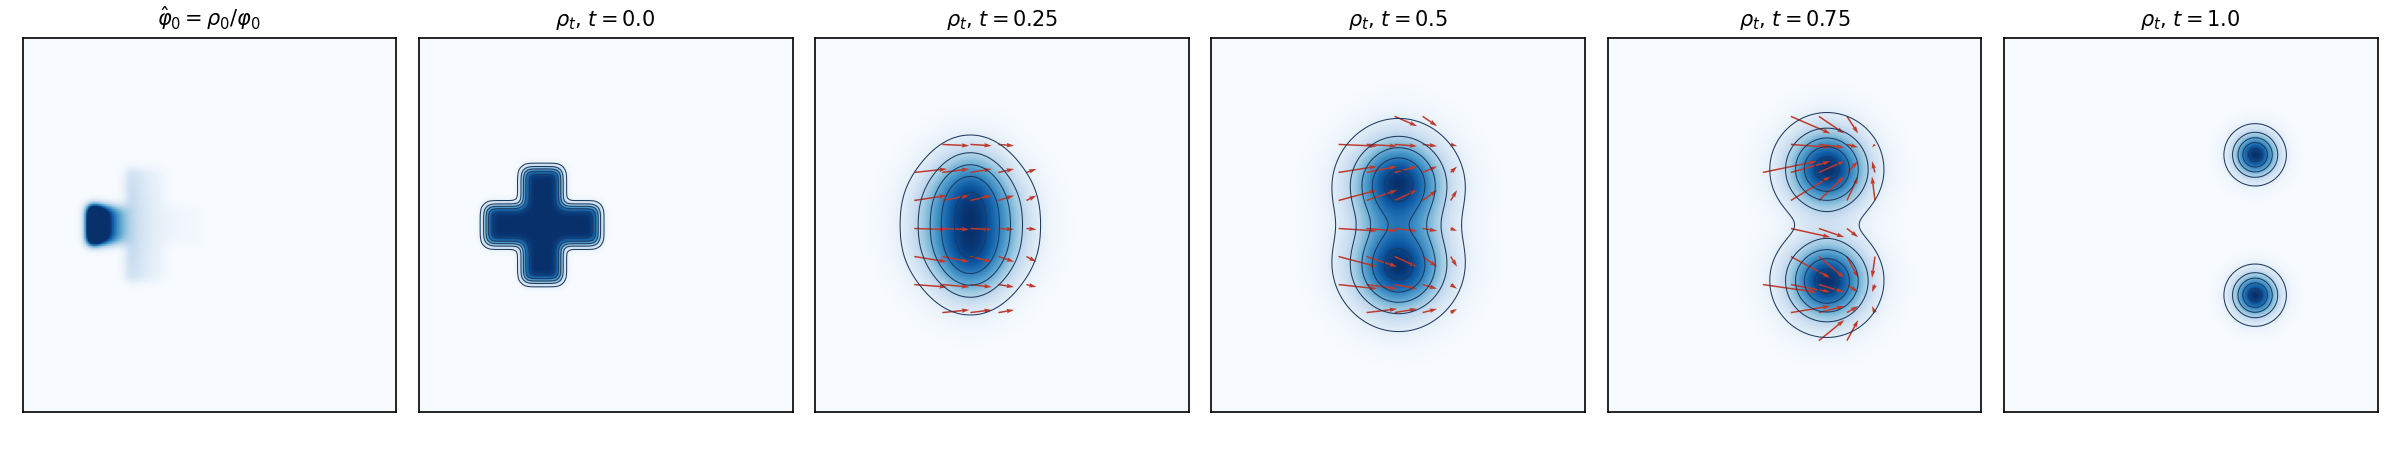
\includegraphics[width=\textwidth]{figures/cross_sb_2d.png}
\caption{Plus-sign to two blobs, $\eps=0.01$, all from the Recipe~A reference (no solver
run). Left: the forced factor $\hphi$, concentrated on the arm facing away from the targets.
Then $\rho_t$ at $t=0,\tfrac14,\tfrac12,\tfrac34,1$ with the closed-form drift as arrows;
contours at 10--90\% of each panel's peak.}
\label{fig:cross}
\end{figure}
  \item \textbf{3D.} \code{example\_split\_3d(eps=0.005)} through \code{3d/} at $n=32,48,64$,
        reference from \code{staggered\_reference(nt=n, ns=(n,n,n))}. The $1\%$ cross branch
        $\Omega_{1,2}=0.006$ is the stress test: check the solver's mass in the region between
        source blob 1 and target $b_2$ at $t=0.75$ against the reference's.
  \item \textbf{Write-up.} One table (grid, $\rho$ error, $m$ error, order, iterations, time)
        per example, the branch-mass check as a short second table, and one figure of
        $\rho_t$ slices with the reference contours overlaid. State the two reference
        error sources (quadrature for Recipe A, box tails for both) with their sizes, so the
        reader knows the reference is $10^4\times$ more accurate than the solver.
\end{enumerate}

\appendix
\section{Answers and hints}
\label{sec:answers}

\paragraph{Ex.\ 1.} $\int\pi\,dy=\hphi(x)\varphi_0(x)$ and $\int\pi\,dx=\hphi_1(y)\varphi(y)$.
Optimality: the entropic plan between two marginals is the unique coupling of the form
$f(x)\Kc_\sigma(x,y)g(y)$ (Schr\"odinger system / Sinkhorn fixed point), so any such
product \emph{is} the optimal plan for the marginals it happens to have.

\paragraph{Ex.\ 2.} $\partial_t\rho=\hphi\partial_t\varphi+\varphi\partial_t\hphi
=-\eps\hphi\Delta\varphi+\eps\varphi\Delta\hphi$. And
$\dv(\rho v)=2\eps\dv(\hphi\nabla\varphi)=2\eps(\nabla\hphi\cdot\nabla\varphi+\hphi\Delta\varphi)$.
Sum: $\eps(\hphi\Delta\varphi+2\nabla\hphi\cdot\nabla\varphi+\varphi\Delta\hphi)=\eps\Delta(\varphi\hphi)$.

\paragraph{Ex.\ 3.} $\varphi_0$: paper's normalizer $Z_x$ (up to a constant), code
\code{phi(0.0,.)}. $\hphi$: never written in the paper; code \code{phihat(0,.)} (Recipe B) or
\code{phihat0} (Recipe A). $\pi^*(y|x)$: paper eq.\ (14) and Prop.\ 3.3; code
\code{conditional\_plan}, \code{conditional\_mixture}. $v$: paper Cor.\ 3.5 eq.\ (16); code
\code{velocity}.

\paragraph{Ex.\ 4.}
\emph{Convolution rule.} Let $X\sim\Nc(\mu,\Sigma)$ and $Y\sim\Nc(0,\tau^2I)$ be
independent. The density of $X+Y$ is the convolution of the two densities. But $X+Y$ is
a linear combination of jointly Gaussian variables, hence Gaussian, with
\[
  \mathbb E[X+Y]=\mu,\qquad
  \operatorname{Cov}(X+Y)=\operatorname{Cov}X+\operatorname{Cov}Y+2\operatorname{Cov}(X,Y)=\Sigma+\tau^2I,
\]
the cross term vanishing by independence. A Gaussian is determined by mean and
covariance, so $\Nc(\cdot;\mu,\Sigma)*\Nc(\cdot;0,\tau^2I)=\Nc(\cdot;\mu,\Sigma+\tau^2I)$.
The same argument with $Y\sim\Nc(\mu_2,\Sigma_2)$ gives the general rule
$\Nc(\cdot;\mu_1,\Sigma_1)*\Nc(\cdot;\mu_2,\Sigma_2)=\Nc(\cdot;\mu_1+\mu_2,\Sigma_1+\Sigma_2)$:
means add and covariances add. Only the $\mu_2=0$ case is needed below, because the heat
kernel has mean zero: $\Kc_\sigma(x,y)=\Nc(y;x,\sigma^2I)$ looks centred at $x$, but $x$ is the
convolution variable, and $\Nc(y;x,\sigma^2I)=\Nc(x-y;0,\sigma^2I)$, so
$\int\Kc_\sigma(x,y)\varphi(y)\,dy=(\Nc(\cdot;0,\sigma^2I)*\varphi)(x)$. Probabilistically the
increment $\sqrt{2\eps}\,W_s$ has mean zero; a nonzero mean would appear only if the reference
SDE had a drift, which would translate every component centre.
(Fourier proof, no probability: the characteristic function of $\Nc(\mu,\Sigma)$ is
$\exp(ik^{\!\top}\mu-\tfrac12k^{\!\top}\Sigma k)$; convolution multiplies transforms, so the
exponents $-\tfrac12k^{\!\top}\Sigma k$ and $-\tfrac12\tau^2|k|^2$ add.)

\emph{Heat flow.} The solution of $\partial_su=\eps\Delta u$, $u(0)=u_0$, is $u(s)=G_s*u_0$
with $G_s(z)=(4\pi\eps s)^{-D/2}e^{-|z|^2/4\eps s}$. Since $4\pi\eps s=2\pi\cdot(2\eps s)$ and
$|z|^2/4\eps s=|z|^2/(2\cdot2\eps s)$, this is $G_s=\Nc(\cdot;0,2\eps sI)$, the density of
$\sqrt{2\eps}\,W_s$ for the reference SDE $dX=\sqrt{2\eps}\,dW$. By the rule with
$\tau^2=2\eps s$, a Gaussian $\Nc(\mu,\Sigma)$ flows to $\Nc(\mu,\Sigma+2\eps sI)$, and by
linearity a mixture flows term by term with unchanged weights.

\emph{Signs.} $\hphi$ runs forward, $\partial_t\hphi_t=+\eps\Delta\hphi_t$, $\hphi_0=\hphi$:
elapsed time $s=t$, so $\hphi_t=\Nc(0,2\eps tI)*\hphi$. $\varphi$ runs backward,
$\partial_t\varphi_t=-\eps\Delta\varphi_t$, $\varphi_1=\varphi$: with $s=1-t$ this is a forward
heat equation started from $\varphi$ at $s=0$, so $\varphi_t=\Nc(0,2\eps(1-t)I)*\varphi$.
Each factor is sharpest at the end where it is prescribed and blurrier away from it.

\emph{Mixtures.}
\[
  \varphi_t(z)=\sum_nw_n\,\Nc\big(z;b_n,Q_n+2\eps(1-t)I\big),\qquad
  \hphi_t(z)=\sum_iu_i\,\Nc\big(z;a_i,P_i+2\eps tI\big).
\]
Two values recur later: $\varphi_0$ (covariances $Q_n+2\eps I$) is the paper's normalizer
$Z_x$; $\hphi_1$ (covariances $P_i+2\eps I$) is what multiplies $\varphi$ to give $\rho_1$.
Using the paper's $\epsilon_{\rm p}=2\eps$ in place of $\eps$ would double both inflations;
the symptom is a reference that fails the finite-difference Fokker--Planck check against our
PDE with coefficient $\eps$.

\paragraph{Ex.\ 5.} Exponent in $z$: $-\tfrac12[z^\top(A^{-1}+B^{-1})z-2z^\top(A^{-1}a+B^{-1}b)]+\dots$,
so precision $C^{-1}=A^{-1}+B^{-1}$ and mean $c=C(A^{-1}a+B^{-1}b)$. Integrating the left side
over $z$ gives $(\Nc(\cdot;0,A)*\Nc(\cdot;0,B))(a-b)=\Nc(a;b,A+B)$.

\paragraph{Ex.\ 6.} $x$-marginal is $\hphi\varphi_0$; set equal to $\rho_0$. Then
$\iint\pi=\int\rho_0=1$.

\emph{The crescent, by hand.} Along the ring's centreline $|x-c|=r$ the density $\rho_0$ is
constant, so the shape of $\hphi=\rho_0/\varphi_0$ there is $1/\varphi_0$. Parametrize
$x(\theta)=c+r(\cos\theta,\sin\theta)$ with $c=(0.35,0.50)$, $r=0.12$. The targets are
$b_\pm=(0.70,0.50\pm0.20)$, and after the backward flow to $t=0$ each has variance
$s^2=0.04^2+2\eps=0.0216$, so $\varphi_0(x)\propto\sum_\pm\exp(-|x-b_\pm|^2/2s^2)$. Write
$b_\pm-c=(\Delta,\pm\eta)$ with $\Delta=0.35$, $\eta=0.20$; then
\[
  |x(\theta)-b_\pm|^2=(r\cos\theta-\Delta)^2+(r\sin\theta\mp\eta)^2
  =r^2+\Delta^2+\eta^2-2r\Delta\cos\theta\mp2r\eta\sin\theta .
\]
The constant drops out of ratios, and the $\sin\theta$ term has opposite signs for the two
targets, so summing the two exponentials gives
\[
  \varphi_0(\theta)\propto e^{\kappa\cos\theta}\cosh(\lambda\sin\theta),\qquad
  \kappa=\frac{r\Delta}{s^2}=1.94,\quad \lambda=\frac{r\eta}{s^2}=1.11,
\]
and therefore
\[
  \hphi(\theta)\propto\frac{e^{-\kappa\cos\theta}}{\cosh(\lambda\sin\theta)} .
\]
The first factor is a von Mises profile around the ring with concentration $\kappa$, peaked
at $\theta=\pi$ (the side facing away from the targets) and smallest at $\theta=0$; the
$\cosh$ factor is even in $\theta$ and only sharpens both. Near-to-far ratio along the
centreline: $e^{2\kappa}=48.9$, which \code{phihat0} reproduces to $10^{-15}$. Across the full
ring width the ratio is larger (the outer edge of the far side is further still from the
targets), which is the factor $261$ quoted in \code{candidate\_3d\_problems.tex}.

\emph{Reading.} $\varphi_0(x)$ is the $\varphi$-weighted probability that a Brownian particle
started at $x$ reaches the targets in unit time. Where that is large the prefactor $\hphi$
must be small for the marginal to stay at $\rho_0$, and vice versa: the crescent is the
correction that keeps the ring uniform although the targets pull on one side. A plot of
\code{phihat0} along the centreline against the formula is a good confirmation, not a
substitute.

\paragraph{Ex.\ 7.} $\exp(-|x-x'|^2/2v)=\exp(-(x_1-x_1')^2/2v)\exp(-(x_2-x_2')^2/2v)$, so the
2D sum over fine cells factorizes into two matrix products. The integrand is a Gaussian of
width $\sqrt{2\eps t}$ times a smooth $\hphi$; at $t=1/32$, $\eps=0.01$, the width is
$0.025$, i.e.\ about $6$ fine cells at $n_f=256$, enough for spectral convergence of the
midpoint rule on a smooth periodic-like integrand (the tails vanish before the box edge).

\paragraph{Ex.\ 8.} Agreement to $\lesssim10^{-9}$ at $n_f\ge256$. The integral of $\hphi_t$
equals that of $\hphi$ up to (i) kernel mass leaving the box and (ii) the discrete kernel's
row sums differing from $1$ by the same midpoint error; both are far below the solver error.

\paragraph{Ex.\ 9.} Product rule with $A=Q_n$ (mean $b_n$), $B=\sigma^2I$ (mean $x$).
``Sampling'': draw $x\sim\rho_0$, pick $n$ with the $x$-dependent weights, draw
$y\sim\Nc(m_n(x),S_n)$. Neural solvers are trained from such pairs and scored by moment
metrics; no density of $\rho_1$ is ever evaluated.

\paragraph{Ex.\ 10.} $\hphi=\rho_0/\varphi_0$ has a \emph{sum} of Gaussians in the
denominator, which is not a Gaussian; its heat flow and the product with $\varphi$ inherit
that.

\paragraph{Ex.\ 11.} The ``any positive pair'' clause of Ex.\ 1. Lose: $\rho_0$ as a free
choice (it becomes an $I\!\cdot\!N$-component mixture). Gain: $\rho_1$, $\rho_t$ explicit,
and the branch-mass table.

\paragraph{Ex.\ 12.} $\int\Kc_\sigma(x,y)\Nc(y;b_n,Q_n)dy=\Nc(x;b_n,Q_n+\sigma^2I)$, then
$\int\Nc(x;a_i,P_i)\Nc(x;b_n,Q_n+\sigma^2I)dx=\Nc(a_i;b_n,P_i+Q_n+\sigma^2I)$. The plan is a
sum of $I\!\cdot\!N$ positive measures, one per $(i,n)$, each a single Gaussian on $\R^{2d}$;
mass is conserved along each branch's bridge, so the mass is the same at every $t$.
The $0.006$ entry: mass sent from the lower source blob to the far upper target $b_2$.

\paragraph{Ex.\ 13.} $A+B=P_i+\sigma^2tI+Q_n+\sigma^2(1-t)I=P_i+Q_n+\sigma^2I$: the $t$'s cancel.

\paragraph{Ex.\ 15.} $v=2\eps\sum_n r_n(t,z)\,(-S_n(t)^{-1}(z-b_n))$ with responsibilities
$r_n\propto w_n\Nc(z;b_n,S_n(t))$. Only $\varphi$ enters; there is no $i$ index. The
$\Omega$-weighted average would be a different vector field (it would depend on $\hphi$).

\paragraph{Ex.\ 16.} $C(t)=\frac{(s^2+\sigma^2t)(s^2+\sigma^2(1-t))}{2s^2+\sigma^2}
=\sigma_g^2+\frac{\sigma^4}{2s^2+\sigma^2}\,t(1-t)$ with $\sigma_g^2=\frac{s^2(s^2+\sigma^2)}{2s^2+\sigma^2}$.
So $2\alpha=\sigma^4/(2s^2+\sigma^2)=4\eps^2/(2s^2+2\eps)$. Eliminating $s^2$:
$\sigma_g^4+\eps^2=\big(\sigma_g^2+\tfrac{2\eps^2}{2s^2+2\eps}\big)^2$ is the identity to verify;
it holds, giving $\alpha=\sqrt{\sigma_g^4+\eps^2}-\sigma_g^2$. Easiest: check numerically
with $s=0.1$, $\eps=0.01$.

\paragraph{Ex.\ 17.} (a) No, pulled toward the targets to $0.342$ because $\varphi_0$
increases toward $x=0.70$. (b) No, narrower ($0.047$): multiplying by $\varphi_0$ adds
precision. (c) Yes, by the up/down symmetry of the design about $y=0.5$.

\end{document}
